\chapter{Função Afim}
		 \section{Atividades Básicas}	
		 	\begin{list}{\textbf{Questão \arabic{quest}.}}{\usecounter{quest}}
%define a margem da lista.	
%\setlength{\labelwidth}{-2mm} \setlength{\parsep}{0mm}
%\setlength{\topsep}{0mm} \setlength{\leftmargin}{-2mm}
\renewcommand{\labelenumi}{(\alph{enumi})}

		 	\item Seja a $f:\mathbb{R}\longrightarrow \mathbb{R}$ definida por $f(x)=4x+1$. Determine:
		 	\begin{multicols}{2}
		 	\begin{enumerate}
		 		\item $f(4)$
		 		\item $f(-2)$
		 		\item $f(-1)+f(0)-f(11)$
		 		\item $2f(3) - f(-3)$
		 	\end{enumerate}
		 	\end{multicols}
		 	
		 	\item Obtenha o domíno de cada função.
		 	\begin{multicols}{2}
		 	\begin{enumerate}
		 		\item $f(x)=9x+3$
		 		\item $g(x)=\displaystyle\frac{x^3 + 8x}{x+3}$
		 		\item $i(x) = \sqrt{x-8}$
		 		\item $j(x)=\displaystyle\frac{\sqrt{x-1}}{x-3}$
		 	\end{enumerate}
		 	\end{multicols}
		 	
		 	\item Dada à função do 1º grau $f(x) = (1 - 5x)$. Determinar:
		 	\begin{multicols}{4}
		 	\begin{enumerate}
		 		\item $f(0)$
		 		\item$f(-1)$
		 		\item $f(1/5)$
		 		\item $f(-1/5)$
		 	\end{enumerate}
			\end{multicols}		 	
		 				
			\item Considere a Função do 1º Grau $f(x) = -3x + 2$. Determine os valores de $x$ para que se tenha:
			\begin{multicols}{3}
			\begin{enumerate}
				\item $f(x) = 0$
				\item $f(x) = 11$
				\item $f(x) = -1/2$
			\end{enumerate}
			\end{multicols}
			
			\item Dada a função $f(x) = (ax + 2)$, determine o valor de a para que se tenha $f(4) = 22$.
			\item Dada a função $f(x) = ax + b$ e sabendo-se que $f(3) = 5$ e $f(-2) = -5$ calcule $f(1/2)$.
			\item Um vendedor recebe mensalmente um salário composto de duas partes: uma parte fixa, no valor de \$ 1.000,00 e uma parte variável que corresponde a uma comissão de 18\% do total de vendas que ele fez durante o mês.
				\begin{enumerate}
					\item Expressar a função que representa seu salário mensal.
					\item Calcular o salário do vendedor durante um mês, sabendo-se que vendeu \$ 10.000,00 em produtos.
				\end{enumerate}. 
			\item Em uma determinada loja, o salário mensal fixo de um vendedor é de R\$ 240,00. Além disso, ele recebe R\$ 12,00 por unidade vendida.
		\begin{enumerate}
			\item Expresse o ganho mensal (S) desse vendedor em função do número (u) de unidades vendidas.
			\item Quantas unidades ele deve vender para receber um salário de R\$ 700,00?
			\item Determine o domínio e a imagem desta função
		\end{enumerate}
		
		\item Um comerciante teve uma despesa de \$ 230,00 na compra de certa mercadoria. Como vai vender cada unidade por \$ 5,00, o lucro final L será dado em função das x unidades vendidas. Responda:
		\begin{enumerate}
		 	\item Qual a lei dessa função f;
		 	\item Para que valores de x têm f(x) < 0? Como podemos interpretar esse caso?
		 	\item Para que valores de x haverá um lucro de \$ 315,00?
		 	\item Para que valores de x o lucro será maior que \$ 280,00?
		\end{enumerate}
		
%+==========================================================================================
	\item Sendo $f(x) = x - 3$ e $g(x) = -3x + 4$, determine: 
	\begin{multicols}{3}
	\begin{enumerate}
		\item $f(f(0))$
		\item $g(g(2))$
		\item $f(f(0)) + g(g(2))$
	\end{enumerate}
	\end{multicols}		
	\item Esboce o gráfico da função sobre os números reais $f(x)  = 2x + 3$. 	
	\item Determine o domínio $D$ da função:
	\begin{multicols}{3}	
	\begin{enumerate}
		\item $f(x)=10x+5$
		\item $f(x)=\displaystyle\frac{2}{x}$
		\item $f(x)=\displaystyle\frac{1}{x-3}$
		\item $f(x)=\sqrt{x}$
		\item $f(x)=\sqrt{x+3}$
		\item $f(x)=\displaystyle\frac{3}{\sqrt{x-2}}$
	\end{enumerate}
	\end{multicols}	
	
	\item Determine se cada um dos gráficos abaixo representa uma função:
	\begin{multicols}{2}
	\begin{enumerate}
		\item 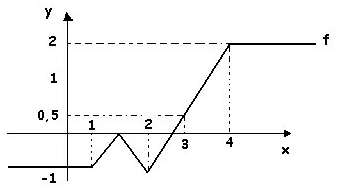
\includegraphics[scale=0.6]{figuras/fig10}
		\item 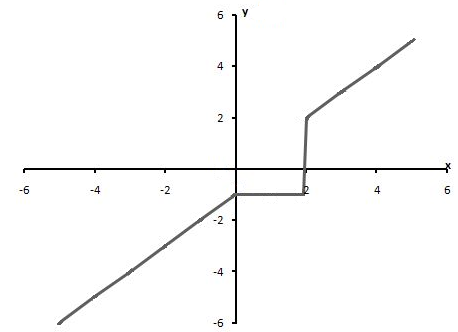
\includegraphics[scale=0.4]{figuras/fig11}
		\item 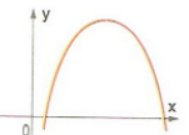
\includegraphics[scale=0.9]{figuras/fig12}
		\item 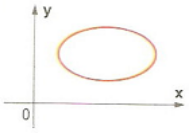
\includegraphics[scale=0.9]{figuras/fig13}			
	\end{enumerate}
	\end{multicols}	
	
	\item Na produção de peças, uma indústria tem um custo fixo de R\$ 8,00 mais um custo variável de R\$ 0,50 por unidade produzida. Sendo $x$ o número de unidades produzidas:
	\begin{enumerate}
		\item Escreva a lei da função que fornece o custo total de x peças;
		\item Calcule o custo de 100 peças;
		\item Escreva a taxa de crescimento da função.
	\end{enumerate}
	\item Na revelação de fotos, uma empresa calcula o preço a ser cobrado usando uma fórmula $P=12,00 + 0,65n$, onde $P$ é o preço, em reais, a ser cobrado e $n$ o número de fotos reveladas.
	\begin{enumerate}
		\item Quanto pagarei se forem reveladas 22 fotos?
		\item Se paguei a quantia de R\$ 33,45 pela revelação, qual o total de fotos reveladas?
	\end{enumerate}
		 		\item A cetesb detectou uma certa companhia jogando ácido sulfúrico no Rio Tiete, multou-a em \$ 125.000,00, mais \$ 1.000,00 por dia até que a companhia se ajustasse às normas legais que regulamentam os índices de poluição. Expresse o total de multa como função em numero de dias em que a companhia continuou violando as normas. 
		 		
		 		\item Em algumas cidades você pode alugar um carro \$ 154 por dia mais um adicional de \$ 16,00 por km. Determine a função por um dia e esboce no gráfico. Calcule o preço para se alugar por um dia e dirigi-lo por 200 km.
		 		
		 		\item Uma companhia de gás irá pagar para um proprietário de terra \$ 15.000,00 pelo direito de perfurar a terra para encontrar gás natural, e \$ 0,3 para cada mil pés cúbicos de gás
extraído. Expresse o total que o proprietário irá receber com função da quantidade de gás
extraído. Esboçar o gráfico.

				\item Em 1998, um paciente pagou \$ 300,00 por um dia em um quarto de hospital semiprivativo e \$ 1.500,00 por uma operação de apêndice. Expresse o total pago pela cirurgia como função do número de dias em que o paciente ficou internado.

				\item O preço a ser pago por uma corrida de táxi inclui uma parcela fixa, denominada bandeirada, e uma parcela que depende da distância percorrida. Se a bandeirada custa R\$ 5,50 e cada quilômetro rodado custa R\$ 0,90, calcule:

				\begin{enumerate}
					\item o preço de uma corrida de 10 km.
					\item a distância percorrida por um passageiro que pagou R\$ 19,00 pela corrida.	
				\end{enumerate}

16. As funções consumo e poupança de um operário de renda variável y são, respectivamente, $C = 100 + 0,6y$ e $S = 0,4y-100$.
				\begin{enumerate}
					\item Qual o seu consumo e sua poupança se ele ganhar R\$ 480,00?
					\item Qual o seu consumo se sua renda for nula? Como você explica a existência de consumo com uma renda nula?	
					\item Qual a sua poupança se sua renda for nula? Como você explica a existência de poupança negativa?
				\end{enumerate}

				\item Na revelação de um filme, uma ótica calcula o preço a ser cobrado usando a fórmula $P = 12,00 + 0,65n$, onde $P$ é o preço,em reais, a ser cobrado e $n$ o número de fotos reveladas do filme.
				\begin{enumerate}
					\item Quanto pagarei se forem reveladas 22 fotos do meu filme?
					\item Se paguei a quantia de R\$ 33,45 pela revelação, qual o total de fotos reveladas?
				\end{enumerate}


				\item O preço a ser pago por uma corrida de táxi inclui uma parcela fixa, denominada bandeirada, e uma parcela que depende da distância percorrida. Se a bandeirada custa R\$ 3,44 e cada quilômetro rodado custa R\$ 0,86, calcule:

				\begin{enumerate}
					\item o preço de uma corrida de 11 km;
					\item a distância percorrida por um passageiro que pagou R\$ 21,50 pela corrida.
				\end{enumerate}

				\item Um fabricante usa como política de vendas, colocar seu produto ao início de janeiro ao preço $p$ e aumentar mensalmente esse preço de 3,00. Em 1 de setembro esse preço passou a R\$ 54,00. Nestas condições determinar:
				\begin{enumerate}
					\item O preço inicial em janeiro
					\item Qual será o preço em dezembro
					\item Esboçar o gráfico da função que rege o preço do produto
				\end{enumerate}

		 	\end{list}	
		 	
	 	\section{Questões de Vestibular}
							
				\begin{center}
				\uppercase{Texto para próxima questão.}
				\end{center}
				Da  frieza  dos  números  da  pesquisa  saíram algumas recomendações. Transformadas em políticas públicas, poderiam reduzir a gravidade e as dimensões da tragédia urbana do trânsito. A   primeira é a adoção de práticas que possam reduzir a gravidade dos acidentes.A segunda     recomendação trata dos motociclistas, cuja frota equivale a 10\% do total, mas cujos custos   correspondem   a   19\%.O 'motoboy' ganha R\$2 por entrega, a empresa, R\$8. É um exército de garotos em disparada. O pedestre forma o contingente  mais vulnerável  no  trânsito  e  necessita  de  maior  proteção, diz a terceira recomendação da pesquisa. Entre a 0h e  as  18h  da  quinta-feira,  as  ambulâncias  vermelhas do  Resgate  recolheram  16  atropelados  nas  ruas  de São Paulo.
				
Fonte: "Folha de São Paulo", com adaptações
			\begin{list}{\textbf{Questão \arabic{quest}.}}{\usecounter{quest}}
%define a margem da lista.	
%\setlength{\labelwidth}{-2mm} \setlength{\parsep}{0mm}
%\setlength{\topsep}{0mm} \setlength{\leftmargin}{-2mm}
\renewcommand{\labelenumi}{(\alph{enumi})}

				\item  Conforme o texto, num dia de trabalho, são necessárias 12 entregas para um motoboy receber R\$24,00. Por medida de segurança, a empresa limitará a 10 a quantidade de entregas por dia. Como compensação, pagará um adicional fixo de p reais ao dia a quem atingir esse limite, porém reduzirá para R\$1,80 o valor pago por cada entrega. O valor de p que manterá inalterada a quantia diária recebida pelo motoboy, ou seja, R\$24,00, será:
				\begin{multicols}{5}				
				\begin{enumerate}
					\item R\$ 5,40
					\item R\$ 5,60
					\item R\$ 5,80
					\item R\$ 6,00
					\item R\$ 6,20
				\end{enumerate}
				\end{multicols}
				
				\begin{center}
				\uppercase{Texto para as próximas duas questões.}
				\end{center}
				(Faap) Medições realizadas mostram que a temperatura no interior da terra aumenta, 
aproximadamente, 3$^o$C a cada 100m de profundidade. Num certo local, a 100m de profundidade, a temperatura é de 25$^o$C. Nessas condições, podemos afirmar que:
				\item A temperatura a 1.500m de profundidade é:
				\begin{multicols}{5}
				\begin{enumerate}
					\item 70$^o$C
					\item 45$^o$C
					\item 42$^o$C
					\item 60$^o$C
					\item 67$^o$C
				\end{enumerate}
				\end{multicols}
				
				\item Encontrando-se uma fonte de água mineral a 46$^o$C, a profundidade dela será igual a:
				\begin{multicols}{5}
				\begin{enumerate}
					\item 700 m				
					\item 600 m
					\item 800 m
					\item 900 m
					\item 500 m
				\end{enumerate}								
				\end{multicols}
				
				\begin{center}
					\uppercase{texto para próxima questão.}
				\end{center}				
				(Enem) José Antônio viajarão em seus carros com as respectivas famílias para a cidade de Serra Branca. Com a intenção de seguir viagem juntos, combinam um encontro no marco inicial da rodovia, onde chegarão, de modo independente, ente meio-dia e 1 hora da tarde. Entretanto, como não querem ficar muito tempo esperando um pelo outro, combinam que o primeiro que chegar ao marco inicial esperará pelo outro, no máximo, meio hora; após esse tempo, seguirá viagem sozinho.		
				\item Chamando de $x$ o horário de chegada de José e de $y$ o horário de chegada de Antônio, e representando os pares (x; y) em um sistema de eixos cartesianos, a região OPQR a seguir indicada corresponde ao conjunto de todas as possibilidades para o par $(x, y)$:
				
				\begin{center}
				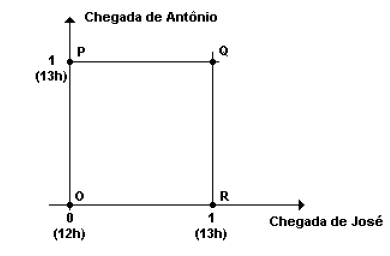
\includegraphics[scale=0.7]{figuras/fig24.png}
				\end{center}
				
				Na região indicada, o conjunto de pontos que representa o evento "José e Antônio chegam ao marco inicial exatamente no mesmo horário" corresponde:
				\begin{multicols}{4}
				\begin{enumerate}
					\item à diagonal OQ
					\item à diagonal PR
					\item ao lado PQ
					\item ao lado QR
					\item ao lado OR
				\end{enumerate}
				\end{multicols}
				
				\begin{center}
				\uppercase{texto para próxima questão.}
				\end{center}
				
				(Faap) A variação de temperatura $y=f(x)$ num intervalo
de tempo $x$ é dada pela função $f(x)=(m^2-9)x^2+(m+3)x+m-3$; calcule "m" de modo que:
				\item O gráfico da função seja uma reta e f(x) seja crescente:
				\begin{multicols}{5}
				\begin{enumerate}
					\item -3
					\item 9
					\item 3
					\item -9
					\item 0
				\end{enumerate}
				\end{multicols}
				
				\item (Mackenzie)
				
				\begin{center}
				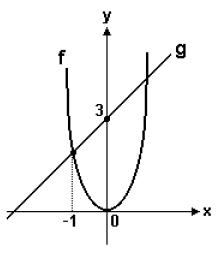
\includegraphics[scale=0.7]{figuras/fig25.png}
				\end{center}
				
				Na figura temos os gráficos das funções $f$ e $g$. Se $f(x)=2x^2$, então $g(3)$ vale:
				\begin{multicols}{5}
				\begin{enumerate}
					\item 6
					\item 8
					\item 10
					\item 12
					\item 14
				\end{enumerate}
				\end{multicols}
				
				\item (Unesp) Considere a função $f:\mathbb{R} \longrightarrow \mathbb{R}$, definida por $f(x)=2x-1$. Determine todos os valores de $m \in \mathbb{R}$ para os quais é válida a igualdade: $$f(m^2)-2f(m)+f(2m)= \displaystyle\frac{m}{2}.$$
				
			    \item (Unesp) Um operário ganha R\$3,00 por hora de trabalho de sua jornada semanal regular de trabalho, que é de 40 horas. Eventuais horas extras são pagas com um acréscimo de 50\%. Encontre uma fórmula algébrica para expressar seu salário bruto semanal, $S$, para as semanas em que trabalhar h horas, com $h\geqslant40$.	
			    
			    \item (Unesp) Uma pessoa obesa, pesando num certo momento 156 kg, recolhe-se a um SPA onde se anunciam perdas de peso de até 2,5 kg por semana. Suponhamos que isso realmente ocorra. Nessas condições:
			    	\begin{enumerate}
			    		\item Encontre uma fórmula que expresse o peso mínimo, P, que essa pessoa poderá atingir após n semanas.
			    		\item Calcule o número mínimo de semanas completas que a pessoa deverá permanecer no SPA para sair de lá com menos de 120 kg de peso.
			    	\end{enumerate}
			
			\end{list}		 	
		\section{Atividades do Enem}				
			\begin{list}{\textbf{Questão \arabic{quest}.}}{\usecounter{quest}}
%define a margem da lista.	
%\setlength{\labelwidth}{-2mm} \setlength{\parsep}{0mm}
%\setlength{\topsep}{0mm} \setlength{\leftmargin}{-2mm}
\renewcommand{\labelenumi}{(\alph{enumi})}
	
				\item 06) (ENEM-08) Uma pesquisa da ONU estima que, já em 2008, pela primeira vez na história das civilizações,a maioria das pessoas viverá na zona urbana. O gráfico a seguir mostra o crescimento da população urbana desde 1950, quando essa população era de 700 milhões de pessoas, e apresenta uma previsão para 2030, baseada em crescimento linear no período de 2008 a 2030.			
				\begin{center}
				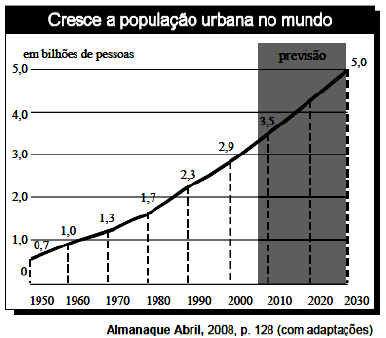
\includegraphics[scale=0.8]{figuras/fig14}
				\end{center}
	De acordo com o gráfico, a população urbana mundial em 2020 corresponderá, aproximadamente, a quantos bilhões de pessoas?
				\begin{multicols}{5}
				\begin{enumerate}
					\item 4,00
					\item 4,10
					\item 4,15
					\item 4,25 
					\item 4,50
				\end{enumerate}
				\end{multicols}
				
				\item (UNIRIO) O valor de um carro popular decresce linearmente com o tempo, devido ao desgaste. Sabendo-se que o preço de fábrica é R\$ 7.500,00 e que, depois de 6 anos de uso, é R\$ 1.200,00, seu valor após 4 anos de uso, em reais é:
				\begin{multicols}{4}
				\begin{enumerate}
					\item 2.100
					\item 2.400
					\item 3.150
					\item 3.300 					 
				\end{enumerate}
				\end{multicols}
				
				\item (UERJ) - Em uma partida, Vasco e Flamengo levaram ao Maracanã 90.000 torcedores. Três portões foram abertos às 12 horas e até as 15 horas entrou um número constante de pessoas por minuto. \newline A partir desse horário, abriram-se mais 3 portões e o fluxo constante
de pessoas aumentou. Os pontos que definem o número de pessoas dentro do estádio em função do horário de entrada estão contidos no gráfico abaixo:
				\begin{center}
				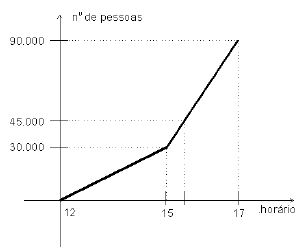
\includegraphics[scale=0.8]{figuras/fig15}
				\end{center}
				Quando o número de torcedores atingiu 45.000, o relógio estava marcando 15 horas e:
				\begin{multicols}{4}
				\begin{enumerate}
					\item 20 min
					\item 30 min
					\item 40 min
					\item 50 min 					 
				\end{enumerate}
				\end{multicols}
				
				\item Um helicóptero desloca-se numa trajetória cuja equação é $y=\displaystyle\frac{1}{2}x+100$. Um míssil disparado contra o helicóptero segue uma trajetória cuja
equação é $y = 2(x -10) + k$. Em ambas as equações,$y$ representa a altura em relação ao eixo $Ox$. O míssil atinge o helicóptero a uma altura de 130 m. Se as distâncias $x$ e $y$ são dadas em metros, o valor de $k$ será:
				\begin{multicols}{4}
				\begin{enumerate}
					\item 0
					\item 10
					\item 20
					\item 30 					 
				\end{enumerate}
				\end{multicols}


			\end{list}	

